
\begin{figure}
    \centering
    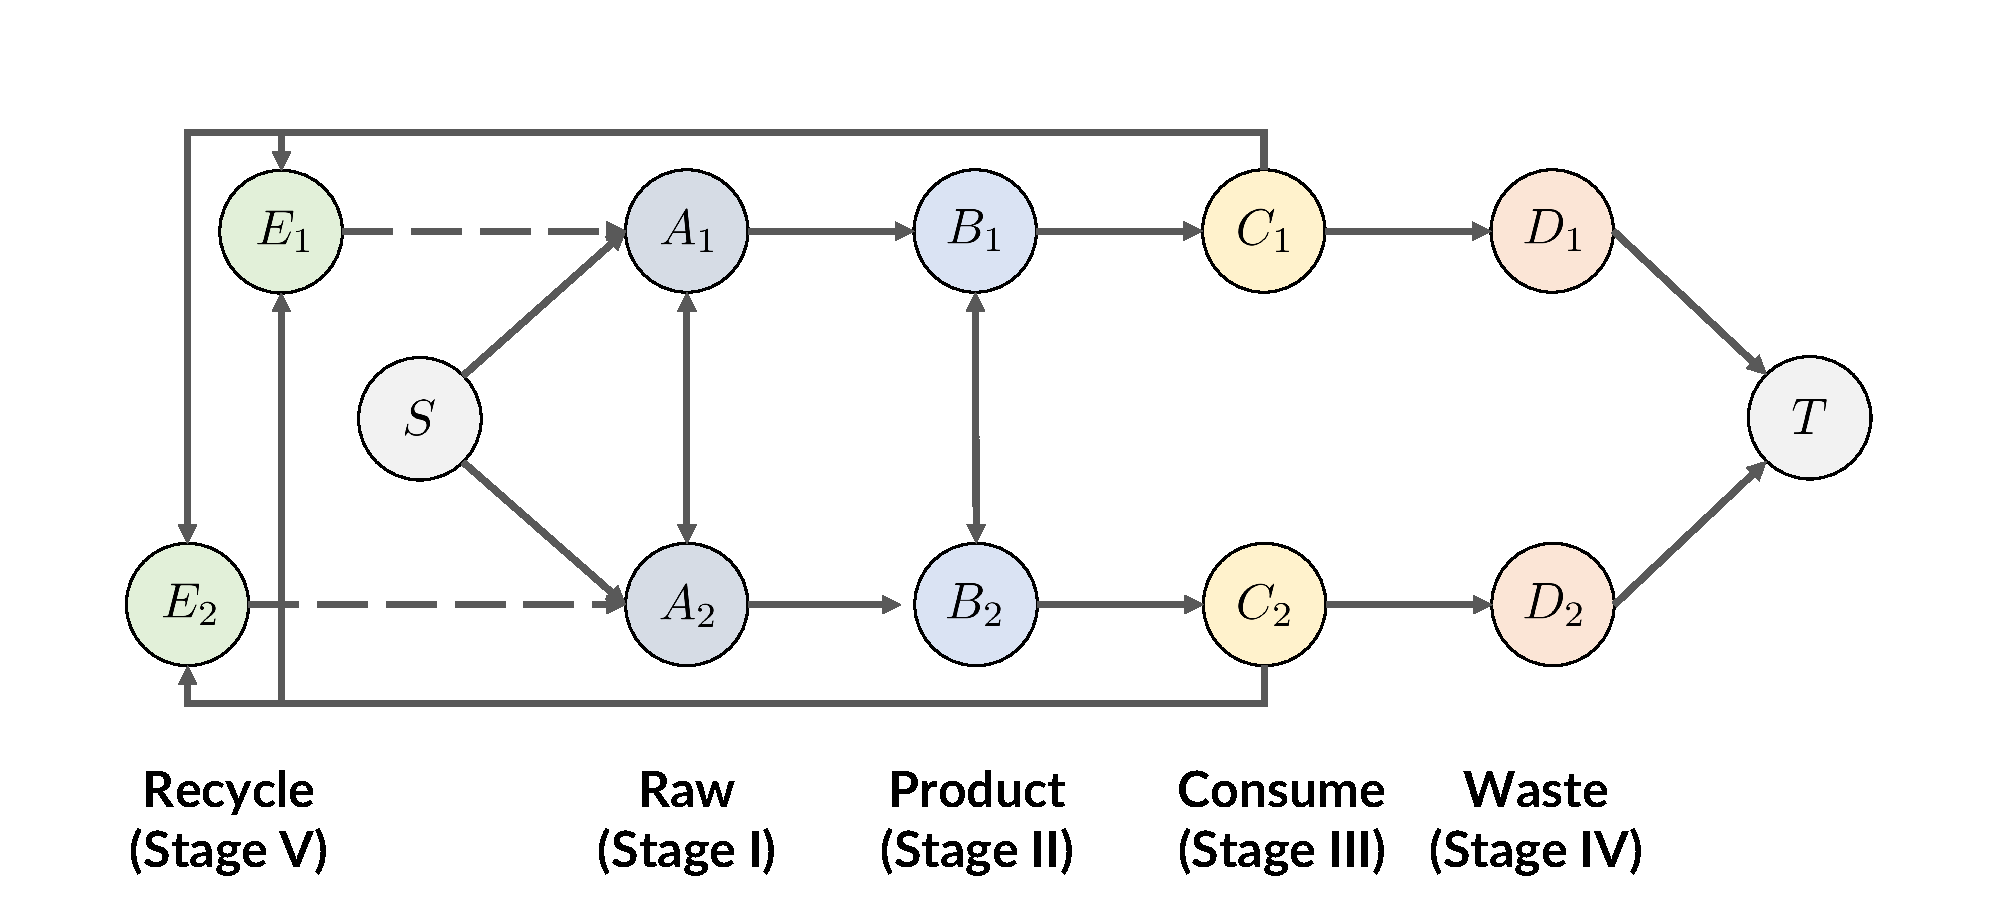
\includegraphics[width=0.6\textwidth]{figures/data-open-flow-model.pdf}
    \caption{The plastic network flow model within the economy of two countries, including production (\textbf{Stages I, II}), consumption (\textbf{Stage III}), waste (\textbf{Stage IV}), and recycling (\textbf{Stage V}). Our model applies to more countries in the world and can be extended to more stages.}
    \label{fig:flow-model}
\end{figure}

In this subsection, we describe a method used to find optimal production, trade, and recycling allocations that minimizes certain metrics of plastic pollution. Our method is related to the concept of network flow problems in optimization theory; we optimize for the flow that describes the allocations of production, trade, and recycling, while satisfying constraints on production, trade, recycling, and consumption based on real-world data.  

\subsubsection{Stages of plastic flow and problem statement}
We consider the life cycle of a unit of plastic particle that enters and leaves the world economy via the following stages:
\begin{description}
    \item [\textbf{Stage I}] Raw forms of plastic are created from fossil fuel and related precursors; this stage mostly depends on the countries' fossil fuel supply. International trade can happen at this stage to balance supply and demand.
    \item [\textbf{Stage II}] Manufactured goods that contains plastic as a component are created from raw forms of plastic, possibly via intermediate forms of plastics; this stage mostly depends on the countries' industrial production capacity. International trade can happen at this stage to balance supply and demand. We note that this also considers products that has plastic as a component but are not primarily plastic. 
    \item [\textbf{Stage III}]
    Plastic waste are produced as a result of consumption of manufactured goods; this stage mostly depends on the countries' consumption capacity.
    \item [\textbf{Stage IV}]
    A part of the plastic waste are managed domestically, and mis-managed plastic waste (MMPW) are produced as a result; this stage depends on the countries' ability to collect and handle plastic waste properly (such as by recycling).
    \item [\textbf{Stage V}] The remaining plastic waste are managed through international trade, where the importer of plastic waste will either recycle the plastic for its own use or dispose of it (which may lead to increased pollution from the importer). This stage is subject to supply, demand, and certain domestic policies (such as tariffs and import bans). We assume that the recycled plastic particles will become raw forms of plastic (\textbf{Stage I}) that can be reused in production.
\end{description}
International trade happens at \textbf{Stages} \textbf{I}, \textbf{II} and \textbf{V}. We are interested in designing trade policies happening at these stages that benefit the environment while keeping our standard of living. 
To this end, we make two assumptions to our model: 
\begin{description}
    \item[\textbf{Assumption I}] Our trade policies will not reduce consumption of manufactured goods at \textbf{Stage III}.  
    \item[\textbf{Assumption II}] Countries will not import plastic waste at \textbf{Stage V} unless said waste will be used for recycling.
\end{description}

\subsubsection{Network flow model of plastic}

Now we are ready to describe our method as solving a minimum cost maximum flow problem on a directed acyclic graph (DAG) $G = (\mathcal{V}, \mathcal{E})$. The nodes (vertices) $\mathcal{V}$ represents the countries at certain stages and edges $\mathcal{E}$ represents the transition to certain stages (production, consumption, trade, or waste disposal). Edges additionally have two properties: \textit{capacity}, which describes an upper limit for the possible \textit{plastic flow} through the edge (\textit{e.g.}, production, consumption, or trade), and \textit{cost}, which describes the environmental cost efficiency\footnote{We also use the term ``cost'' for conciseness.} of the edge (\textit{e.g.}, waste disposal). We note that the cost efficiency is over each unit of plastic; if the cost efficiency for one countries' waste disposal is 0.5, then we mean that one unit of plastic waste will generate 0.5 unit of mis-managed plastic waste.

Let $n$ be the total number of countries in the world (indexed $1$ to $n$). We use the notations $A_i, B_i, C_i, D_i, E_i$ to denote nodes of a country indexed $i$ for each respective stage.
The nodes and edges are defined as follows:
\begin{description}
    \item[\textbf{Stage I}] First, we define $n$ ``production'' edges from a source node $S$ to every $A_i$, with cost being small and capacity depending on the countries' capacity to produce raw plastic materials. Then, we define $n(n-1)$ ``trade'' edges between $A_i$ and $A_j$, with cost being small and capacity depending on the export limit of raw plastic materials from country $i$ to country $j$.
    \item[\textbf{Stage II}] First, we define $n$ ``production'' edges from $A_i$ to $B_i$, with cost being small and capacity being the industrial capacity to create products from the raw plastic materials.  Then, we define $n(n-1)$ ``trade'' edges between $B_i$ and $B_j$ ($i \neq j$), with cost being small and capacity depending on the export limit of products from country $i$ to country $j$. 
    \item [\textbf{Stage III}] We define $n$ ``consumption'' edges from $B_i$ to $C_i$, with cost being zero and capacity being the consumption capacity of country $i$. There is no trade at this stage.
    \item [\textbf{Stage IV}] We define $n$ ``waste'' edges from $C_i$ to $D_i$, with cost depending on the rate of creating mismanaged plastic (MMPW) and capacity being infinite. This stage models the process of plastic waste being discarded, as well as plastic waste that are not recovered during the recycling process.
    We can modify the cost to optimize different metrics of plastic pollution, such as total MMPW on the planet, in a specific country, or the total MMPW that results in ocean pollution. Following common practices in network flow definitions, we also define $n$ edges between each $D_i$ and a sink node $T$ with zero cost and infinite capacity. There is no trade at this stage.
    \item [\textbf{Stage V}] We define $n^2$ ``recycle'' edges from $C_i$ to $E_j$ ($i$ can be equal to $j$) with cost being zero and capacity being infinity. We further define $n$ edges between $E_j$ to $A_j$ for each country $j$, with cost being zero and capacity being the country's maximum amount to recycle plastic. This naturally also sets an upper limit to the capacity over the ``recycle'' edges. 
\end{description}


Given the definition of the DAG, we can see the life cycle of a unit of plastic via a path from $S$ to $T$ (Figure~\ref{fig:example})
\begin{description}
    \item[Type I: Not recycled] The unit of plastic is produced, consumed and discarded in country $i$.
    $$S \xrightarrow{\mathrm{raw}} A_i \xrightarrow{\mathrm{product}} B_i \xrightarrow{\mathrm{consume}} C_i \xrightarrow{\mathrm{waste}} D_i \to T$$
    \item[Type II: Recycled] The unit of plastic is produced and consumed in country $i$, but recycled by country $j$ via international trade; then it is produced, consumed, and discarded in country $j$.
    $$S \to A_i \to B_i \to C_i \xrightarrow{\mathrm{traded}} E_j \xrightarrow{\mathrm{recycled}} A_j \to B_j \to C_j \to D_j \to T$$
    We note that this path can be extended as long as there are countries willing to recycle the unit of plastic from $j$.
\end{description}
Here, we see that in \textbf{Type II}, one unit of plastic satisfies one unit of consumption in both countries $i$ and $j$, which is impossible in \textbf{Type I}. Our \textbf{Assumption II} also ensures that the traded plastic waste will be recycled and used again in consumption.

\begin{figure}
\centering
\begin{subfigure}{0.47\textwidth}
    \centering
    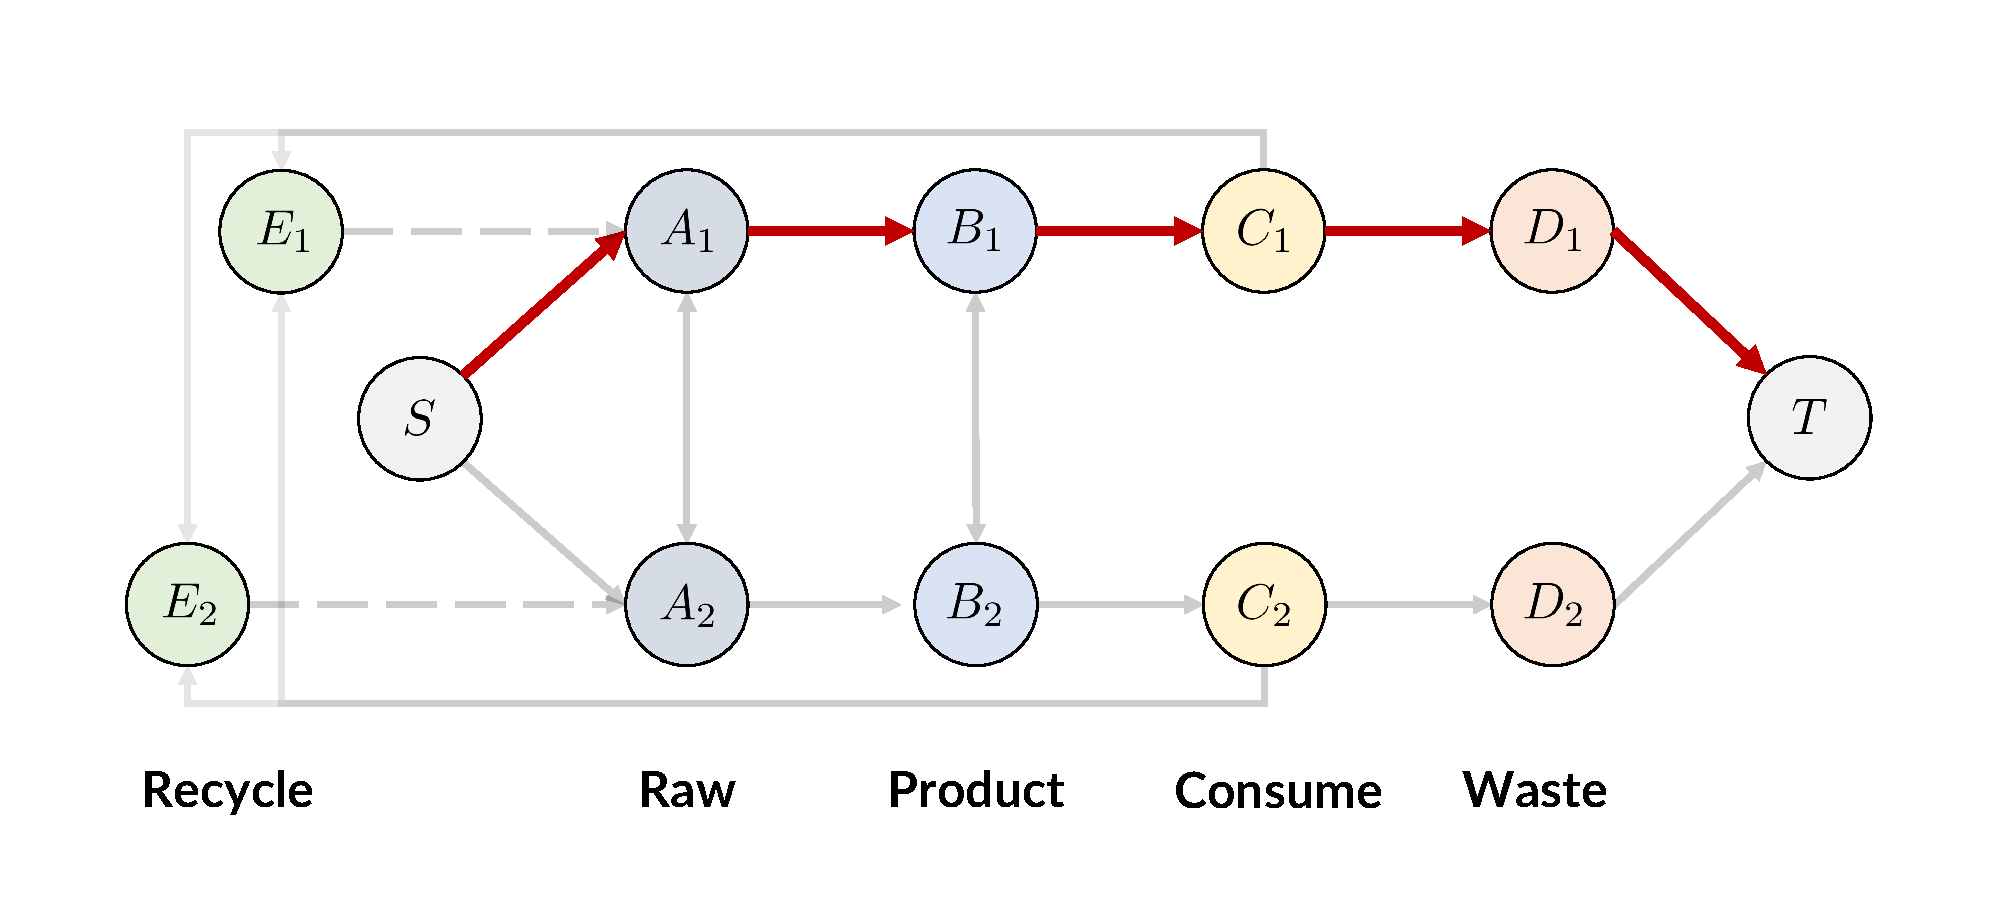
\includegraphics[width=\textwidth]{figures/data-open-type_1.pdf}
    \caption{Type I: Not recycled.}
\end{subfigure}
~
\begin{subfigure}{0.47\textwidth}
    \centering
    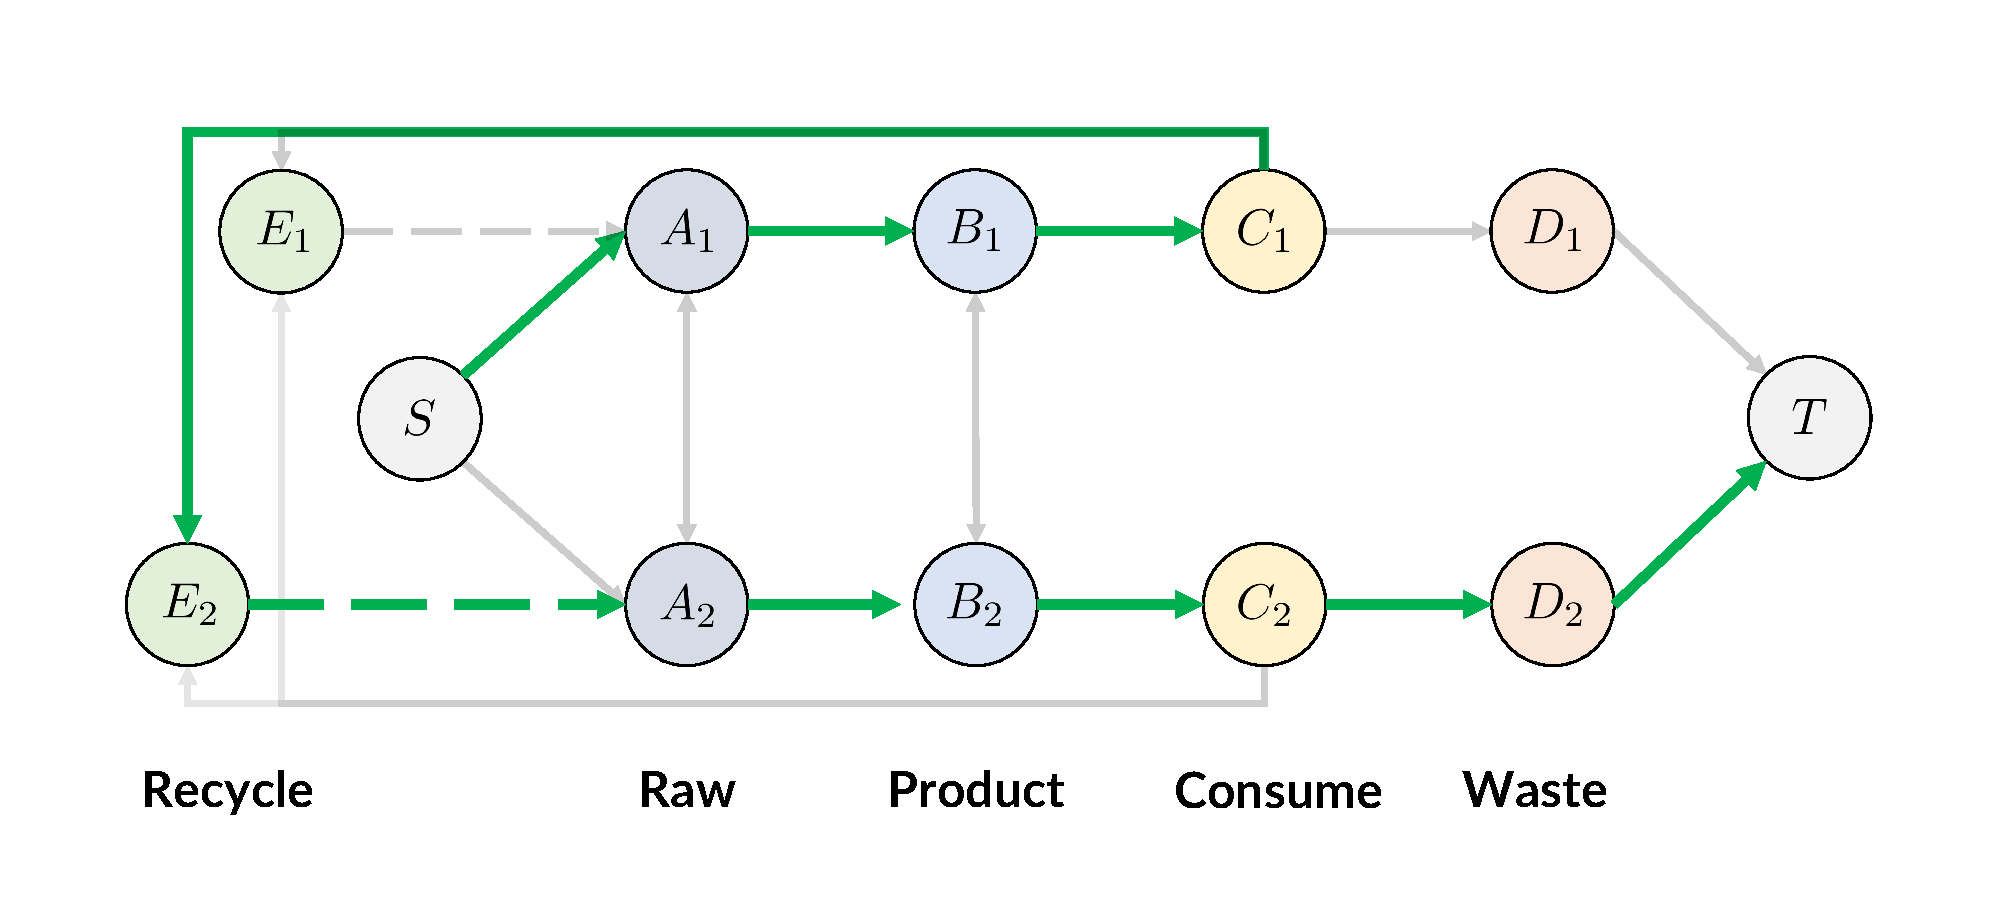
\includegraphics[width=\textwidth]{figures/data-open-type_2.pdf}
    \caption{Type II: Recycled.}
\end{subfigure}
\caption{The flow of one unit of plastic; the plastic can be either discarded directly (a, red path) or recycled (b, green path). With recycling, one unit of plastic can satisfy two units of consumption.}
\label{fig:example}
\end{figure}

\subsubsection{Objective function}
We can define an objective over the trade assignments in \textbf{Stages} \textbf{I}, \textbf{II}, and \textbf{V}; as well as production, consumption, and discard stages. We describe this as a non-negative \textit{flow} function $f: \mathcal{E} \to \mathbb{R}_{\geq 0}$ over edges.
We can then optimize the flow function $f$ to reduce plastic pollution. Our goal is to minimize the amount of pollution, defined via the cost in the edges:
\begin{align}
    L(f) := \sum_{e \in \mathcal{E}}^{n} f(e) \cdot \mathrm{cost}(e)
\end{align}
where $\mathrm{cost}: \mathcal{E} \to \mathbb{R}$ is a cost function that captures a measure of pollution on each unit of plastic through the edge (\textit{e.g.}, cost of discarding one ton of plastic). The feasible solutions should satisfy the following constraints:
\begin{description}
\item[\textbf{Constraint I}] Flow does not exceed capacity, \textit{i.e.},
    $
    \forall e \in \mathcal{E}, f(e) \leq \mathrm{cap}(e),
    $
    where $\mathrm{cap}: \mathcal{E} \to \mathbb{R}$ is the capacity function that we defined to model the constraints at each edge.
    \item[\textbf{Constraint II}] Except for $S$ and $T$, every node has same amount of inflow and outflow.
    $
    \forall v \in \mathcal{V} \setminus \{S, T\}, \sum_{e \in \mathcal{E}} f(e) I(v, e) = 0
    $
    where $I: \mathcal{V} \times \mathcal{E} \to \{-1, 0, +1\}$ is a function that takes value $+1$ if $v$ is the receiving node of $e$, $-1$ if $v$ is the sending node of $e$, and $0$ if $v$ is not a node on the edge $e$.
    \item[\textbf{Constraint III}] Consumption capacities are satisfied for every country, \textit{i.e.},
    $
    \forall i \in [n], f(B_i \to C_i) = \mathrm{cap}(B_i \to C_i),
    $
    where instead of the usual inequality constraints, here we use the equality constraint.
\end{description}
We note this defines a linear program over $f$ where methods such as interior point algorithms can be applied. To maximize computational efficiency of the optimization problem, however, we leverage algorithms on minimum cost maximum flows that are guaranteed to give exact optimal solutions in polynomial time for integer cost and constraints\footnote{When costs and constraints are floats, multiplying them with a large number and then converting to integer often suffices.}, as well as a binary search method to find the optimal flow $f^\star$ that minimizes impact on the environment while satisfying consumption needs (details in Appendix \ref{app:binsearch}).

\subsection{Parameters of the plastic flow}

We can simulate different scenarios (\textit{e.g.}, trade limits) by setting different capacity functions $\mathrm{cap}$ and cost functions $\mathrm{cost}$. As our interest is primarily on the effect from plastic waste trade, we set the following edge values for all our experiments\footnote{Unless specified, costs are zero (as we mostly focus on plastic pollution) and capacities are infinity.}:
\begin{itemize}
    \item The total consumption $F_{\mathrm{tot}}$ over the world is derived from yearly plastic production, measured in tons per year\footnote{Source: \href{https://ourworldindata.org/grapher/global-plastics-production}{[Our World in Data: Global Plastics Production]}.}.
    % 
    \item The capacities of countries' supply of raw plastic materials (\textbf{Stage I}) are distributed according to oil supply in each country, \textit{i.e.}, $\mathrm{cap}(S \to A_i) = \{\mathrm{oil\ supply\ of\ } i\} \times F_{\mathrm{tot}} / \{\mathrm{global\ oil\ supply}\}$; the sum of all supplies is $1.2 F_{\mathrm{tot}}$.
    \item The capacities of countries' production of products that consist of plastics (\textbf{Stage II}) are distributed according to industrial GDP in each country, \textit{i.e.}, $\mathrm{cap}(A_i \to B_i) =  \{\mathrm{industrial\ GDP\ of\ } i\} \times F_{\mathrm{tot}} / \{\mathrm{global\ industrial\ GDP}\}$; the sum of all production is $1.1 F_{\mathrm{tot}}$.
    \item The capacities of countries' consumption of products (\textbf{Stage III}) are distributed according to (nominal) GDP in each country, \textit{i.e.}, $\mathrm{cap}(B_i \to C_i) = \{\mathrm{GDP\ of\ } i\} \times F_{\mathrm{tot}} / \{\mathrm{global\ GDP}\}$; the sum of all consumption is $F_{\mathrm{tot}}$.
    \item The capacities of countries' disposal of products (\textbf{Stage IV}) are infinite, but the cost is mismanaged plastic waste rate, i.e., $\mathrm{cost}(C_i \to D_i) = \{\mathrm{mismanaged\ plastic\ waste\ generation\ of\ } i\} / \{\mathrm{plastic\ waste\ generation\ of\ }i\}$. We use the average mismanaged plastic waste rate to impute the countries without the data.
\end{itemize}
Our main focus is over international trade on plastic waste, which are reflected in the capacities of the following edges:
\begin{description}
\item[Trade capacities] The capacities over countries' trade of plastic waste $\mathrm{cap}(C_i \to E_j)$ (\textbf{Stage V}) are proportional to the real-world trade data in metric tons. The details about how we obtain the trade volume between the countries are described in ref{sec:data}. These can be influenced more directly by a country's trade policies.
\item[Recycling capacities] The capacities over countries' ability to recycle plastic waste $\mathrm{cap}(E_j \to A_i)$ (\textbf{Stage V}) are proportional to the countries' GDP per capita. These depend more on the technology level of the country, and are less sensitive to trade policies.
\end{description}
To control the capacities, we often multiply a constant hyperparameter over all the base capacities derived from data.
We may also increase or decrease these capacities for individual countries to simulate different trade scenarios. 